% CAPÍTULO 23 — «O relógio e a causa» (andar 1: o que não se compra, começando pela experiência)
% Fracasso que o abre: o capítulo da queda conjunta deixou \numConjuntaAssimetria{} de assimetria a
% \numConjuntaDesvios{} desvios do nulo --- e o leitor escreve sozinho «o índice americano puxa o
% Ibovespa». Os dois mercados não partilham o dia: a sessão de um e a do outro são janelas de
% vinte e quatro horas que se sobrepõem, e a ordem pode ser o RELÓGIO. Este capítulo mede as três
% contas que separam a ordem da causa: o alinhamento declarado, o canal impossível e o terceiro
% comum. Caderno: E37_relogio_causa (semente 104, quarenta nulos, varredura de menos dois a mais
% dois dias). Veredito: a assimetria não sobrevive ao relógio declarado (+0,69 desvios), cresce no
% alinhamento cronológico verdadeiro (+2,99), não se repete sem canal (-0,15 e +0,94) e não
% aparece sem seta (de -0,85 a +0,40). A ordem é o relógio.
% Figuras: figuras/E37_relogio_1.pdf (a varredura contra o nulo deslocado) e
% figuras/E37_relogio_2.pdf (o terceiro comum contra a linha do par real).
% Costuras: o fecho do 22 entrega a experiência que o leitor pediu; a nota de parte ganha a
% experiência que não se compra; a abertura do 24 reconhece o andar já aberto.

\chapter{O relógio e a causa}\label{cap:relogio}

\section{A frase que o leitor escreve sozinho}

O capítulo anterior terminou com uma ordem de pé: dos episódios dirigidos entre o índice americano
e o Ibovespa, a assimetria é \numConjuntaAssimetria, a \numConjuntaDesvios{} desvios do nulo,
positiva nas janelas e nos pedaços. A frase que qualquer leitor escreve na linha seguinte é «o
índice americano puxa o Ibovespa». É uma frase de causa, e o capítulo não a mediu --- mediu ordem.

O problema é que os dois mercados não partilham o dia. A sessão americana e a sessão brasileira são
duas janelas de vinte e quatro horas que se sobrepõem sem coincidir: uma fecha antes da outra, e o
que é «o mesmo dia» para uma não é para a outra. A ordem medida pode ser o \textbf{relógio} --- a
posição das janelas --- e não a causa. E o número que decide isto não estava impresso em capítulo
nenhum: este capítulo não podia imprimi-lo antes de medi-lo. Agora pode.

\section{O alinhamento declarado, e o nulo que o carrega}

O instrumento é o mesmo do capítulo anterior, com a mesma regra dos episódios dirigidos e a mesma
janela de \numConjuntaJanelaEpisodio{} dias. O que muda é o \emph{par}: cada dia de uma série é
reencontrado com outro dia da outra, deslocado por um número declarado de dias --- os valores são
os mesmos, os rompimentos são os mesmos, o que troca é quem encontra quem. O alinhamento do relógio
declarado é o que a frase causal pede: o índice americano de ontem contra o Ibovespa de hoje, as
mesmas vinte e quatro horas.

E o nulo viaja junto. O capítulo do orçamento já ensinou que este instrumento tem viés próprio, e
que o número do par real só vale contra pares sorteados com a mesma regra; aqui a regra inclui o
deslocamento --- cada nulo sorteado passa pelo mesmo reencontro de dias antes da medida. Sem isso a
régua seria de outro desenho, e o pico da varredura poderia ser do instrumento. A varredura vai de
menos dois a mais dois dias, com \numRelogioNulos{} nulos por ponto e a dispersão entre eles junto.

\section{A ordem que não sobrevive ao relógio}

\begin{figure}[ht]
\centering
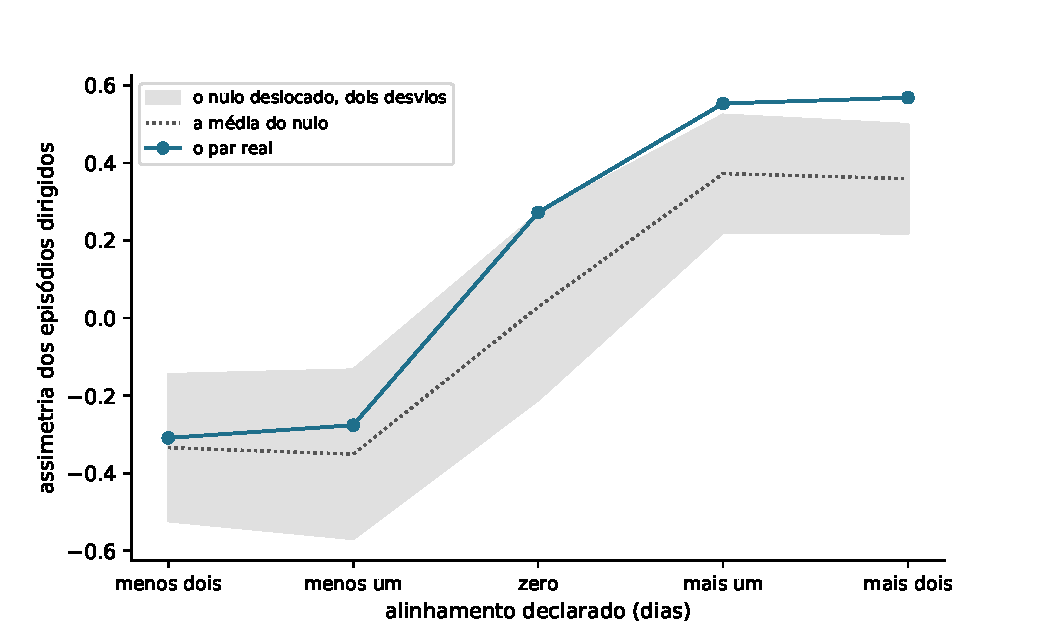
\includegraphics[width=\textwidth]{figuras/E37_relogio_1.pdf}
\caption{A assimetria dos episódios dirigidos no par real, contra o alinhamento declarado --- com a
faixa de dois desvios do nulo deslocado em cada ponto. No alinhamento do relógio declarado (menos
um: o índice de ontem contra o Ibovespa de hoje) a assimetria troca de sinal e cai ao nulo; no
alinhamento que dá ao Ibovespa a vantagem cronológica (mais um e mais dois) ela cresce acima de
dois desvios. A ordem segue o head start, não a causa.}
\label{fig:relogio_varredura}
\end{figure}

No alinhamento de sempre, o par real mede \numRelogioZeroAssimetria{} de assimetria a
\numRelogioZeroDesvios{} desvios --- a casa do número do capítulo anterior, re-medida com os nulos
deste caderno. No alinhamento do relógio declarado, o número desaba: \numRelogioMenosUmAssimetria,
a \numRelogioMenosUmDesvios{} desvios --- ruído. A frase «o índice americano puxa o Ibovespa no dia
seguinte» é exatamente o alinhamento onde a assimetria deixa de existir.

E no alinhamento oposto ela cresce: o Ibovespa de ontem contra o índice de hoje mede
\numRelogioUmAssimetria{} a \numRelogioUmDesvios{} desvios, e \numRelogioDoisAssimetria{} a
\numRelogioDoisDesvios{} com dois dias. Quem recebe a vantagem cronológica é quem lidera. A
sessão brasileira fecha antes da americana no mesmo dia útil; quando o reencontro de dias dá ao
Ibovespa essa posição de quem já fechou, o «líder» é ele. A ordem que o capítulo anterior mediu não
sobrevive ao relógio: ela \emph{é} o relógio.

\section{O canal impossível}

Falta separar o que é janela do que é dependência genérica. O Bitcoin negocia vinte e quatro horas
por dia, sete por semana: sessão nenhuma em comum com qualquer um dos dois mercados --- um par sem
canal nenhum para a história da sobreposição. O mesmo instrumento, o mesmo nulo, o atraso zero:
contra o índice, \numRelogioBtcSpDesvios{} desvios; contra o Ibovespa, \numRelogioBtcIbovDesvios{} desvios.
Nenhum dos dois pares sem canal repete a assinatura. O que escreveu a frase do leitor não é
dependência qualquer: é a estrutura das sessões --- e sem a sobreposição, a assimetria não aparece.

\section{O terceiro que puxa os dois}

\begin{figure}[ht]
\centering
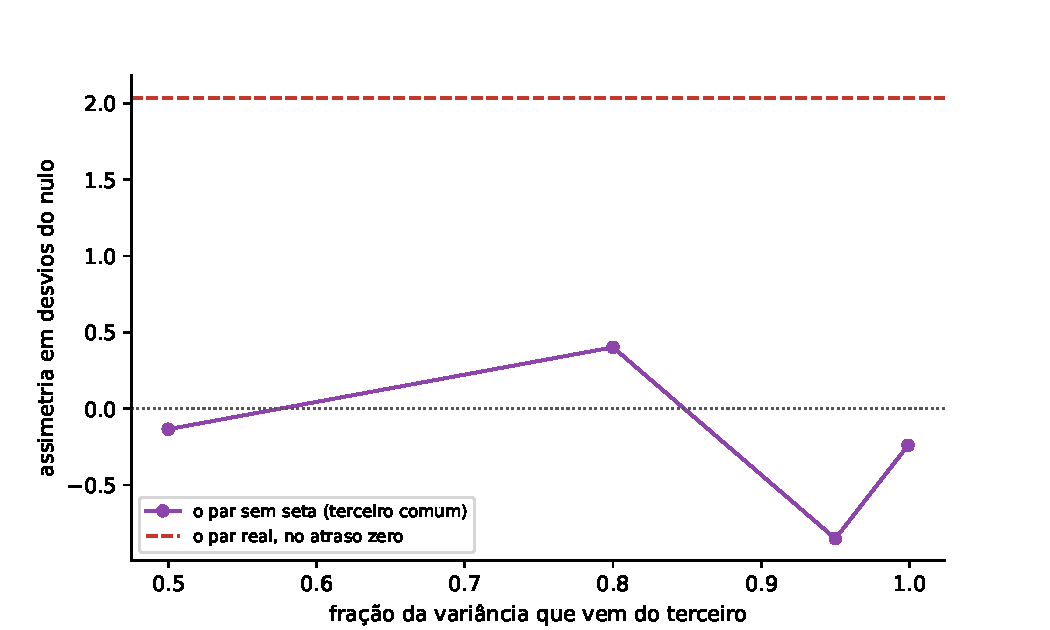
\includegraphics[width=\textwidth]{figuras/E37_relogio_2.pdf}
\caption{A assinatura em desvios do par sem seta --- duas pernas independentes movidas por um
terceiro comum, com as margens do par real --- contra a fração da variância que vem do terceiro. A
linha tracejada é o par real no atraso zero. Em nenhuma fração o par sem seta alcança a linha: a
confusão sozinha não escreve a frase.}
\label{fig:relogio_terceiro}
\end{figure}

O outro candidato a escrever a frase sem causa é a confusão: um terceiro que puxa os dois
\cite{pearl2000bayesian}. Dois mundos são sorteados --- pernas independentes entre si, movidas por
um choque comum declarado, com as margens do par real (índice a \numRelogioTerceiroSigmaSp,
Ibovespa a \numRelogioTerceiroSigmaIbov, \numRelogioTerceiroDias{} dias) --- e a fração da
variância que vem do terceiro sobe de \numRelogioTerceiroMeioDesvios{} desvios na metade, a
\numRelogioTerceiroAltoDesvios{} em quatro quintos, a \numRelogioTerceiroMuitoAltoDesvios{} perto
do um e a \numRelogioTerceiroQuaseUmDesvios{} no quase-um. Em nenhum ponto o par sem seta alcança o
par real. A perna menos ruidosa rompe antes, é verdade --- mas isso fica longe de escrever a
frase do leitor. A confusão sozinha não explica a assinatura das sessões.

\section{A perna que falta: a cascata}

O capítulo separou relógio de causa com o terceiro que puxa os dois --- o fator comum. Sobrou uma
perna que essa família não constrói: o dia em que B rombeu \textbf{porque} A rombeu, a falha que se
propaga de uma perna à outra \cite{buldyrev2010catastrophic} --- a cascata que não precisa de
designer nenhum \cite{bak1987self}, e a que o próprio projeto fabrica quando otimiza demais a
tolerância \cite{carlson1999highly}.

O desenho é o da casa: dois mundos com os \numRelogioDoisDias{} dias do par, calibrados para a
mesma contagem conjunta na janela de três dias e para as mesmas marginais declaradas --- no choque,
o fator rompe as duas pernas no mesmo dia; na cascata, A rombe por conta própria e transmite a B
com a probabilidade calibrada de \numCascataTransmissaoCalibrada, depois de um lag declarado entre
zero e dois dias; a taxa própria de B é ajustada para a marginal casar --- e casa até a aproximação
do ajuste em duas passadas: \numCascataChoqueB{} rompimentos de B no choque contra
\numCascataCascataB{} na cascata, diferença declarada. A calibração da contagem fecha:
\numCascataChoqueConjuntas{} conjuntas no choque contra \numCascataCascataConjuntas{} na cascata.
Em contagem, são o mesmo mundo.

\begin{figure}[htbp]
  \centering
  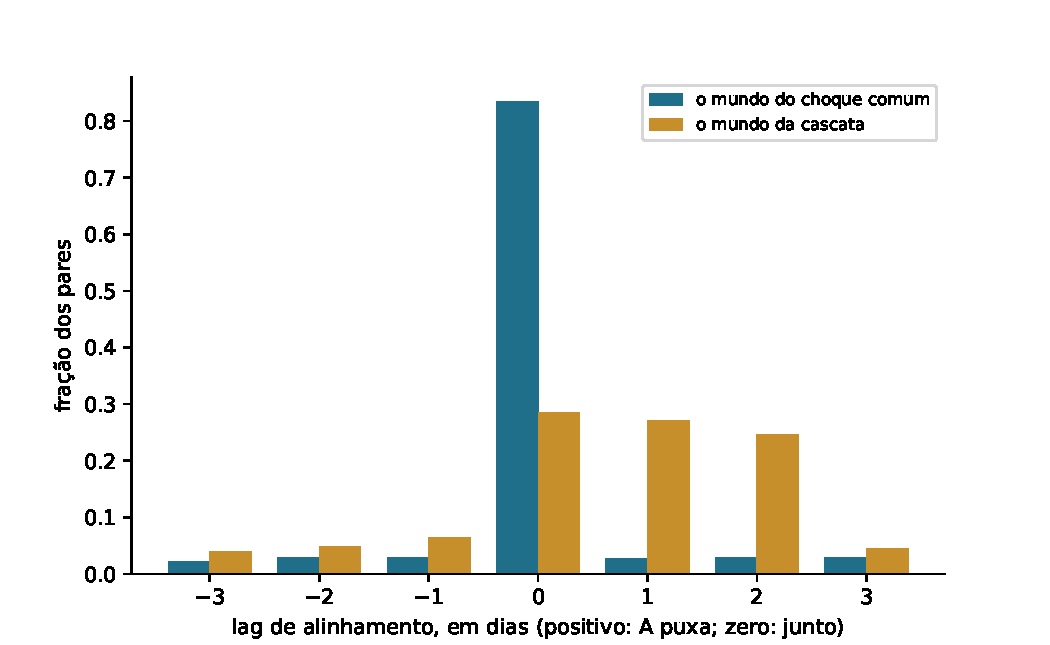
\includegraphics[width=\linewidth]{figuras/E42_cascata_1.pdf}
  \caption{Os histogramas de alinhamento dos dois mundos, na mesma contagem conjunta. O choque
    concentra quase tudo no zero; a cascata espalha entre o zero, o um e o dois --- o atraso da
    propagação é visível no alinhamento. O que o histograma não devolve é a fração de B que
    depende de A: esse número não mora em nenhuma barra.}
  \label{fig:cascata_alinhamento}
\end{figure}

E aqui está a divisão do trabalho entre as leituras. O alinhamento \textbf{vê o atraso}: a fração
dos pares no lag zero é \numCascataLagZeroChoque{} no choque contra \numCascataLagZeroCascata{} na
cascata, e a assimetria média vai de \numCascataAssimetriaChoque{} a \numCascataAssimetriaCascata{}
--- quem olha o histograma sabe que há propagação. Mas nenhuma leitura observacional devolve
\textbf{quanto} de B depende de A: a fração transmitida não está no alinhamento, nem na contagem,
nem na marginal --- só existe do lado de quem corta.

A intervenção é o corte: bloquear os rompimentos de A e contar os de B. No choque, o bloqueio mata
\numCascataChoqueMortas{} rompimentos de B --- zero, porque nenhuma perna deve nada à outra; o
fator seguiria disparando com A calado. Na cascata, \numCascataCascataMortas{}
[\numCascataCascataMortasMin{}; \numCascataCascataMortasMax{}] dos rompimentos de B morrem com o
bloqueio --- dois quintos deles. Esse número, e nenhum outro, é a medida da dependência: e é o
preço que a seção seguinte cobra, na moeda dela.

\begin{figure}[htbp]
  \centering
  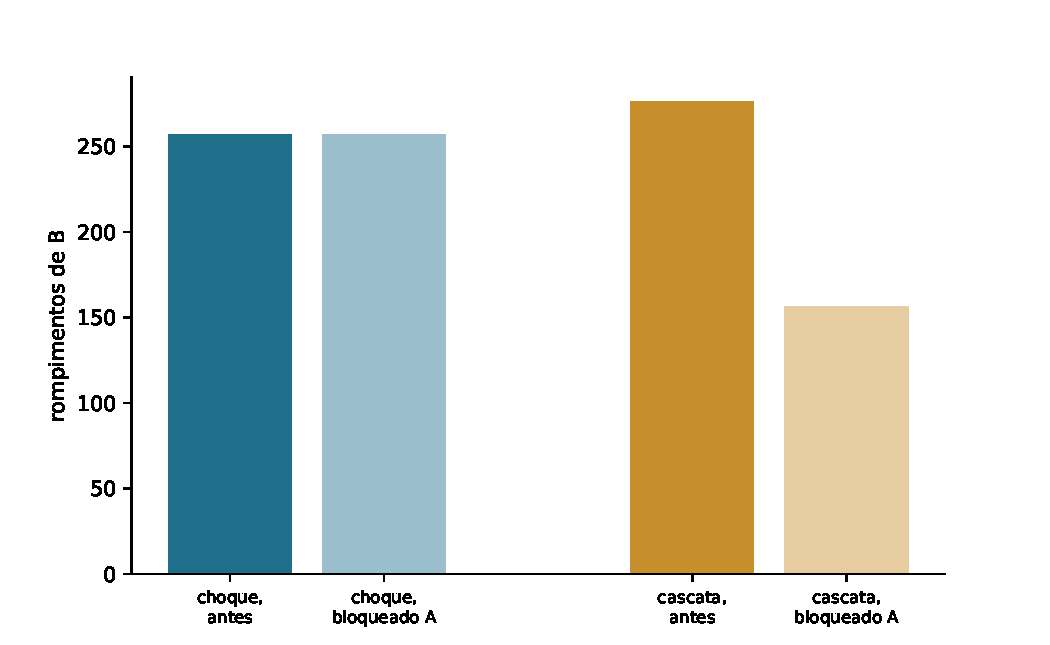
\includegraphics[width=\linewidth]{figuras/E42_cascata_2.pdf}
  \caption{A intervenção: os rompimentos de B antes e depois do bloqueio de A, nos dois mundos. A
    barra clara do choque não desce --- zero mortas; a da cascata desce quase à metade: a fração
    que dependia de A, que nenhum alinhamento devolvia.}
  \label{fig:cascata_intervencao}
\end{figure}
\section{O preço, na moeda da intervenção}

As três contas fecham na mesma direção, e cada uma morre de um jeito: a ordem não sobrevive ao
relógio; a dependência sem canal não a produz; a confusão sem seta não a alcança. O que ficaria de
pé, para sustentar a frase de causa, é a intervenção --- o experimento que segurasse um mercado e
observasse o outro \cite{pearl2000bayesian, wang2025causal}. Esse experimento existe para uma
rede, para uma planta, para um serviço; para um mercado, não existe de jeito nenhum, e os quadros
de identificação que a literatura desenha pedem exatamente aquilo que aqui não se compra
\cite{kim2025causal}. A primeira coisa que o andar coloca fora de qualquer compra é esta
experiência. O que sobra é declarar: a ordem medida é o relógio das sessões, a frase de causa não
tem quem a pague, e a conta mais dura do andar ainda nem começou --- a de uma proteção calibrada no
mundo que não se viu.